% !TeX program = xelatex
% 脑机协同康复机械臂闭环可视化系统 —— 产品说明书
% 编译：xelatex 说明书.tex （跑两遍以生成目录）

\documentclass[11pt, a4paper]{ctexart}

\usepackage{geometry}
\geometry{top=2.4cm, bottom=2.4cm, left=2.6cm, right=2.6cm}

\usepackage{graphicx}
\usepackage{xcolor}
\usepackage{booktabs}
\usepackage{tabularx}
\usepackage{longtable}
\usepackage{array}
\usepackage{amsmath}
\usepackage{caption}
\usepackage{subcaption}
\usepackage{enumitem}
\usepackage{fancyhdr}
% 本机 TeX Live 缺 pdfcol.sty（tcolorbox 的依赖），改用 mdframed + TikZ 后端做提示框
\usepackage[framemethod=TikZ]{mdframed}
\usepackage{hyperref}

% ---------- 配色：取自应用本身的设计令牌 ----------
\definecolor{brand}{HTML}{16A394}      % 主色 · 青绿
\definecolor{brandink}{HTML}{16323F}   % 正文深色
\definecolor{brandsoft}{HTML}{EAF6FB}  % 浅底
\definecolor{brandline}{HTML}{B7D3E4}  % 分隔线
\definecolor{brandgrey}{HTML}{7F96A5}  % 次要文字
\definecolor{warn}{HTML}{D97706}       % 提示橙

\hypersetup{
  colorlinks=true,
  linkcolor=brand,
  urlcolor=brand,
  citecolor=brand,
  pdftitle={脑机协同康复机械臂闭环可视化系统 · 产品说明书},
  pdfauthor={揭榜挂帅参赛团队},
}

% ---------- 章节名：第 N 章 ----------
\ctexset{
  section = {
    name = {第,章},
    number = \arabic{section},
    format = \Large\sffamily\bfseries\color{brandink},
    beforeskip = 1.6ex plus 0.4ex minus 0.2ex,
    afterskip = 1.0ex plus 0.2ex,
  },
  subsection = {
    format = \large\sffamily\bfseries\color{brandink},
  },
  subsubsection = {
    format = \normalsize\sffamily\bfseries\color{brandink},
  },
}

% ---------- 页眉页脚 ----------
\pagestyle{fancy}
\fancyhf{}
\fancyhead[L]{\small\color{brandgrey}\sffamily 脑机协同康复机械臂闭环可视化系统}
\fancyhead[R]{\small\color{brandgrey}\sffamily 产品说明书}
\fancyfoot[C]{\small\color{brandgrey}\thepage}
\renewcommand{\headrulewidth}{0.4pt}
\renewcommand{\headrule}{\hbox to\headwidth{\color{brandline}\leaders\hrule height \headrulewidth\hfill}}

% ---------- 图注 ----------
\captionsetup{
  font={small},
  labelfont={bf, sf, color=brand},
  textfont={color=brandink},
  labelsep=quad,
  skip=6pt,
}

% ---------- 提示框：左侧色条 + 浅色底，可跨页断开 ----------
\newmdenv[
  backgroundcolor=brandsoft,
  linecolor=brand,
  linewidth=2.5pt,
  leftline=true, rightline=false, topline=false, bottomline=false,
  innerleftmargin=10pt, innerrightmargin=10pt,
  innertopmargin=8pt, innerbottommargin=8pt,
  skipabove=9pt, skipbelow=9pt,
]{keybox}

\newmdenv[
  backgroundcolor=warn!6,
  linecolor=warn,
  linewidth=2.5pt,
  leftline=true, rightline=false, topline=false, bottomline=false,
  innerleftmargin=10pt, innerrightmargin=10pt,
  innertopmargin=8pt, innerbottommargin=8pt,
  skipabove=9pt, skipbelow=9pt,
]{warnbox}

% ---------- 便捷宏 ----------
\newcommand{\shot}[3]{%
  \begin{figure}[htbp]
    \centering
    \includegraphics[width=#2]{figures/#1}
    \caption{#3}
  \end{figure}%
}
\newcommand{\req}[1]{\textcolor{brand}{\sffamily\bfseries #1}}

\renewcommand{\arraystretch}{1.25}

% 手机截图很高（宽高比约 1:2），默认浮动参数会把整页让给一张图，留下大片空白。
% 放宽后允许图与正文同页，排版更紧凑。
\renewcommand{\topfraction}{0.9}
\renewcommand{\bottomfraction}{0.9}
\renewcommand{\textfraction}{0.06}
\renewcommand{\floatpagefraction}{0.8}

% =====================================================================
\begin{document}

% ---------------- 封面 ----------------
\begin{titlepage}
\centering
\vspace*{1.0cm}

{\color{brandgrey}\sffamily\large 揭榜挂帅竞赛参赛作品}

\vspace{0.5cm}
{\color{brandline}\rule{0.35\textwidth}{1.2pt}}
\vspace{0.8cm}

{\sffamily\bfseries\color{brandink}\fontsize{25}{32}\selectfont
脑机协同康复机械臂\\[0.2em] 闭环可视化系统}

\vspace{0.7cm}
{\sffamily\LARGE\color{brand} 产 \; 品 \; 说 \; 明 \; 书}

\vspace{0.45cm}
{\color{brandline}\rule{0.35\textwidth}{1.2pt}}

\vspace{0.9cm}
{\color{brandgrey}\sffamily
脑电信号模拟 \; $\to$ \; 运动意图识别 \; $\to$ \; 光电感知校验 \; $\to$ \; AI 康复决策\\[0.35em]
$\to$ \; 机器人动作响应 \; $\to$ \; 触觉反馈 \; $\to$ \; 训练报告生成}

\vspace{0.8cm}
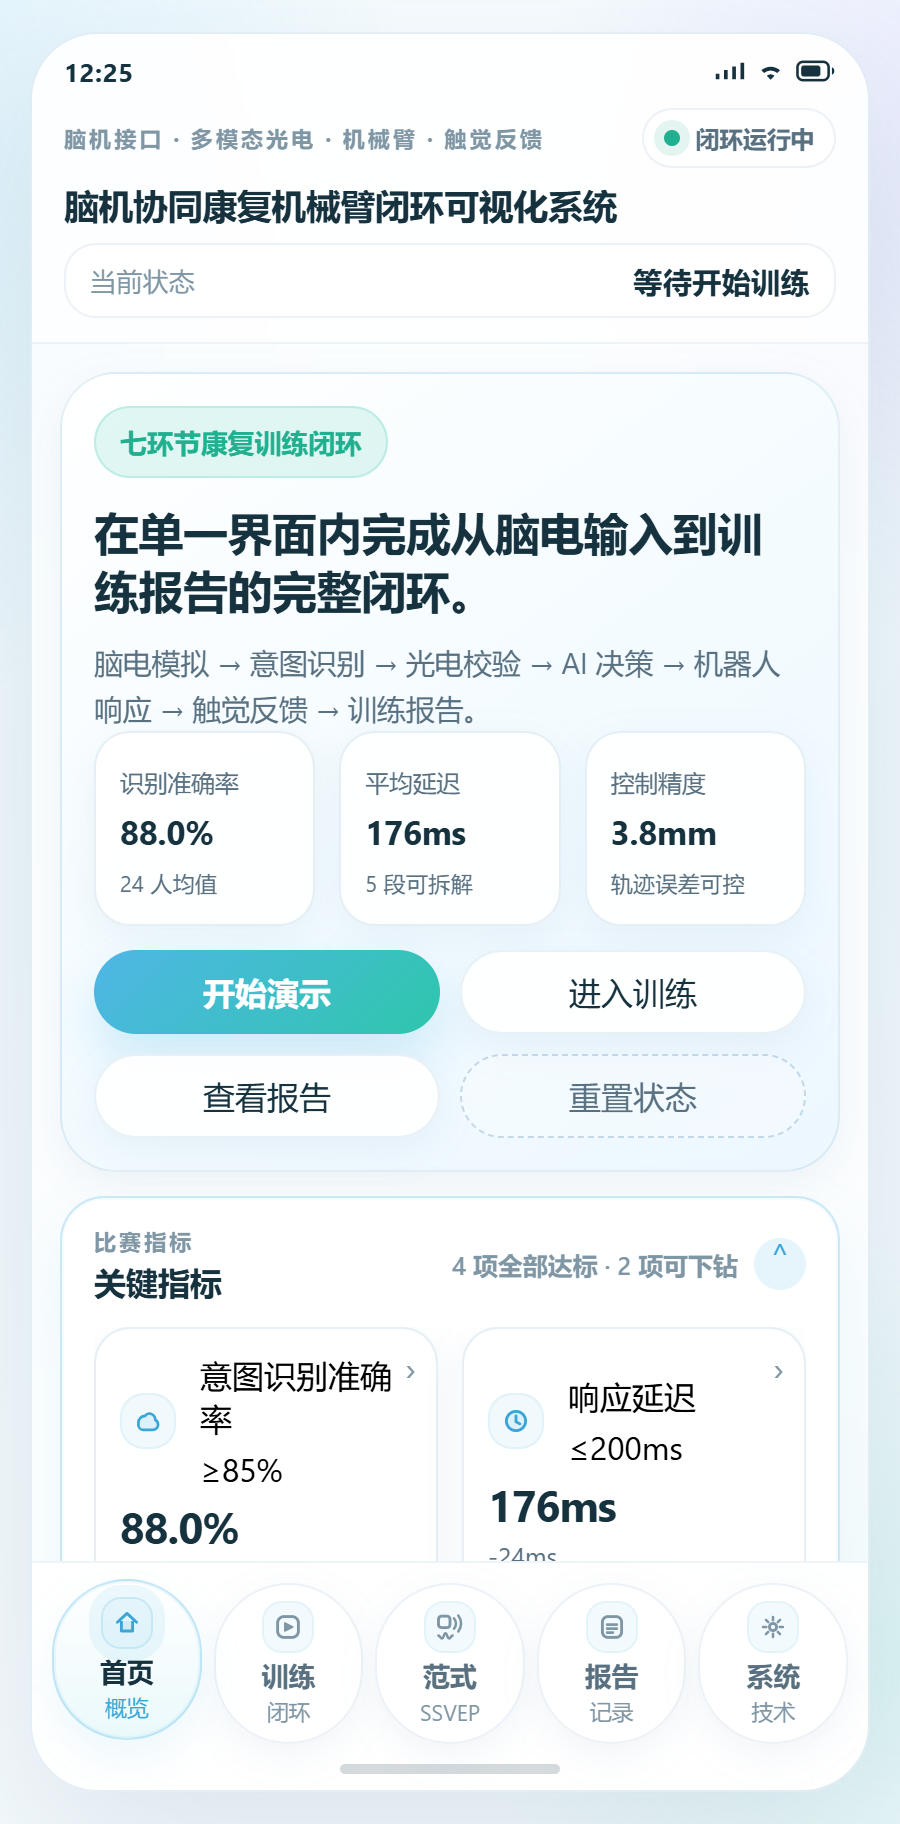
\includegraphics[width=0.245\textwidth]{figures/01-home.png}

\vfill
\begin{minipage}{0.82\textwidth}
\centering\small\color{brandgrey}\sffamily
本说明书所述系统的全部脑电信号与被试队列均为\textbf{仿真合成数据}，\\
用于系统功能验证与竞赛演示，不构成任何临床结论。
\end{minipage}

\vspace{0.7cm}
{\color{brandgrey}\sffamily 版本 v1.0 \quad|\quad 2026 年 7 月}
\end{titlepage}

% ---------------- 目录 ----------------
\tableofcontents
\newpage

% =====================================================================
\section{系统概述}

\subsection{项目定位}

本系统是面向「揭榜挂帅」竞赛的\textbf{脑机接口康复机械臂 APP 原型}。它把一次上肢康复训练从「患者产生运动意图」到「系统给出训练报告」的完整链路，压缩进一块手机屏幕内完成，且每一环节都有独立的可视化与真实的数据联动——上一环的输出即是下一环的输入，不存在只做展示、不参与计算的装饰性面板。

系统解决的核心问题是：\textbf{脑机接口在康复场景中长期停留于「能解码」，却未能证明「解码结果如何安全地驱动机械臂、又如何回到患者的感觉通路」}。本系统以一个七环节闭环回答这一问题，并对个体差异、范式选择与伦理边界给出可核查的工程实现。

\subsection{七环节闭环}

演示流程固定为以下七个环节：

\begin{enumerate}[itemsep=2pt, topsep=4pt]
  \item \textbf{脑电信号模拟}——前额叶通道波形，随意图动态变化；
  \item \textbf{运动意图识别}——抬手 / 伸肘 / 握拳 / 放松四类运动想象，输出置信度与误操作风险；
  \item \textbf{光电感知校验}——RGB / NIR / ToF 三模态交叉校验姿态与轨迹偏差；
  \item \textbf{AI 康复决策}——依据意图、姿态评分、疲劳指数生成训练方案与保护策略；
  \item \textbf{机器人动作响应}——三维机械臂仿真，目标轨迹 / 实际轨迹 / 控制误差实时对比；
  \item \textbf{触觉反馈}——压力、振动、位置感三类反馈，构成感觉运动闭环；
  \item \textbf{训练报告生成}——汇总时长、次数、各项精度指标与康复建议，可导出 Word 文档。
\end{enumerate}

\begin{keybox}
\textbf{闭环的含义。} 第 6 环节的触觉反馈回到患者的\textbf{感觉}通路，与第 1 环节的\textbf{运动}意图共同构成「感觉—运动闭环」；第 7 环节的训练结果又并入个体奖励记忆（第 11 章），影响下一次训练的策略权重。因此本系统是一个\textbf{双重闭环}：单次训练内的感觉运动闭环，与跨训练的个体自适应闭环。
\end{keybox}

\subsection{关键指标}

首页在显著位置展示四项竞赛指标的当前值与达标情况：

\begin{table}[htbp]
\centering
\caption{竞赛关键指标与当前实现值}
\begin{tabularx}{\textwidth}{@{}l c c c X@{}}
\toprule
\sffamily\bfseries 指标 & \sffamily\bfseries 竞赛要求 & \sffamily\bfseries 当前值 & \sffamily\bfseries 余量 & \sffamily\bfseries 可下钻的依据 \\
\midrule
意图识别准确率 & $\ge 85\%$   & 88.0\% & $+3.0\%$   & 24 人队列均值，见第 10 章 \\
响应延迟       & $\le 200$ms  & 176ms  & $-24$ms    & 5 段时延预算，见第 14 章 \\
控制精度       & $\le 5$mm    & 3.8mm  & $-1.2$mm   & 轨迹误差，见第 7 章 \\
抓握力度误差   & $\le 10\%$   & 7.0\%  & $-3.0\%$   & 过力保护钳制，见第 8 章 \\
\bottomrule
\end{tabularx}
\end{table}

\begin{keybox}
\textbf{指标不是孤立数字。} 首页的「意图识别准确率 88.0\%」与「响应延迟 176ms」均可点击下钻：前者跳转至个体支持性页，展示这一数值是如何从 $\sigma = 9.2\%$ 的通用模型收敛而来的；后者跳转至无线采集页，展示 176ms 由哪五个物理环节构成。\textbf{任何一个指标都能追溯到它的构成，而非仅是一个写死的数值。}
\end{keybox}

\shot{01-home.png}{0.40\textwidth}{首页：系统定位、七环节闭环入口与四项关键指标}

\subsection{界面总览}

应用由\textbf{五个主页签}与\textbf{四个技术详情页}构成。

\begin{table}[htbp]
\centering
\caption{界面结构}
\begin{tabularx}{\textwidth}{@{}l l X@{}}
\toprule
\sffamily\bfseries 页面 & \sffamily\bfseries 类型 & \sffamily\bfseries 职责 \\
\midrule
首页 · 概览      & 主页签 & 系统定位、关键指标、闭环入口 \\
训练 · 闭环      & 主页签 & 七环节闭环主流程（本说明书第 3--9 章） \\
范式 · SSVEP     & 主页签 & 反应式脑机接口范式（第 14 章） \\
报告 · 记录      & 主页签 & 训练报告与 Word 导出（第 9 章） \\
系统 · 技术      & 主页签 & 技术结构总览，通向以下四个详情页 \\
\midrule
个体支持性       & 详情页 & 跨被试方差收敛、记忆功能、安抚策略池（第 10--12 章） \\
范式与采集形态   & 详情页 & 主动 / 反应 / 被动式三分法（第 14 章） \\
无线采集与范式形态 & 详情页 & 端到端时延预算分解（第 13--14 章） \\
伦理与安全       & 详情页 & 12 条伦理措施与实现证据（第 15 章） \\
\bottomrule
\end{tabularx}
\end{table}

\shot{05-system.png}{0.40\textwidth}{系统页：技术结构与扩展能力，三个核心能力模块可逐一下钻}

\newpage
% =====================================================================
\section{快速上手}

\subsection{三种运行方式}

\begin{table}[htbp]
\centering
\caption{运行与分发方式}
\begin{tabularx}{\textwidth}{@{}l l X@{}}
\toprule
\sffamily\bfseries 方式 & \sffamily\bfseries 命令 & \sffamily\bfseries 适用场景 \\
\midrule
开发模式   & \texttt{npm run dev}        & 本机开发调试 \\
局域网访问 & \texttt{npm run dev:lan}    & 同一 WiFi 下用手机真机演示 \\
单文件 HTML & \texttt{npm run build:single} & 生成可双击离线打开的单个 HTML，答辩优选 \\
安卓 APK   & \texttt{npm run build:apk}  & 生成 APK，需 Android SDK \\
\bottomrule
\end{tabularx}
\end{table}

\begin{keybox}
\textbf{答辩推荐用单文件 HTML。} \texttt{npm run build:single} 产出的 \texttt{dist-single/index.html} 将 JS 与 CSS 全部内联，双击即可用浏览器打开，\textbf{不依赖任何服务器、不发起任何网络请求}。这既规避了答辩现场网络不可用的风险，也直接构成第 15 章「数据不出端」这一伦理主张的证据。
\end{keybox}

\subsection{标准演示流程}

竞赛答辩请严格按以下顺序操作，全程约 90 秒：

\begin{enumerate}[itemsep=3pt, topsep=4pt]
  \item 在首页点击\textbf{「开始演示」}，系统跳转至训练页并自动推进七个环节；
  \item 若需逐环节讲解，改点\textbf{「手动讲解」}，再用\textbf{「下一步」}逐环推进；
  \item 在环节 2 点击\textbf{「握拳」}意图按钮——EEG 波形、置信度、误操作风险随即联动更新；
  \item 环节 3 自动切换至 ToF 通道，完成光电感知校验；
  \item 环节 4 生成 AI 康复决策方案（辅助抓握 / 标准力度 / 中速执行 / 压力+振动反馈 / 开启过力保护）；
  \item 环节 5 三维机械臂执行「手部抓握」，可拖动旋转视角；
  \item 环节 6 展示压力 / 振动 / 位置感三类触觉反馈，并可点击\textbf{「施加超阈力度」}当场触发过力保护；
  \item 环节 7 生成训练报告，点击\textbf{「导出报告」}下载 Word 文档。
\end{enumerate}

\subsection{深链速查}

在网址后追加参数可直达任意画面，无需逐级点击，适合答辩时快速跳转：

\begin{table}[htbp]
\centering
\caption{深链参数}
\begin{tabularx}{\textwidth}{@{}l X@{}}
\toprule
\sffamily\bfseries 参数 & \sffamily\bfseries 效果 \\
\midrule
\texttt{?tab=demo\&step=N}   & 直达闭环第 N 步（N 取 $1\sim 7$） \\
\texttt{?tab=ssvep}          & SSVEP 反应式范式页 \\
\texttt{?tab=ssvep\&gaze=握拳} & SSVEP 页并预选「握拳」目标 \\
\texttt{?tab=report}         & 训练报告页 \\
\texttt{\#/system/adaptation} & 个体支持性详情页 \\
\texttt{\#/system/wireless}   & 无线采集与时延预算页 \\
\texttt{\#/system/acquisition} & 范式与采集形态页 \\
\texttt{\#/system/ethics}     & 伦理与安全页 \\
\bottomrule
\end{tabularx}
\end{table}

\newpage
% =====================================================================
\section{闭环环节一：脑电信号模拟}

\subsection{功能}

模拟前额叶脑电输入，为后续运动意图识别提供信号基线。面板实时绘制 EEG 波形，并给出\textbf{EEG 通道稳定度 93\%}与当前\textbf{疲劳指数}。

波形并非随机噪声，而是按当前选定意图的振幅、频率、基线偏移三个参数合成——切换意图后波形形态\textbf{立即改变}，这是「脑电波形参与计算、而非仅作装饰」的直接证据。

\begin{table}[htbp]
\centering
\caption{四类意图的脑电波形参数}
\begin{tabular}{@{}l c c c@{}}
\toprule
\sffamily\bfseries 意图 & \sffamily\bfseries 振幅 & \sffamily\bfseries 频率 & \sffamily\bfseries 基线偏移 \\
\midrule
抬手 & 16 & 0.58 & $-4$ \\
伸肘 & 18 & 0.62 & $-1$ \\
握拳 & 22 & 0.78 & \phantom{$-$}0 \\
放松 & 10 & 0.42 & \phantom{$-$}5 \\
\bottomrule
\end{tabular}
\end{table}

\shot{02-demo-step1.png}{0.40\textwidth}{环节一：脑电信号模拟。上方为演示模式切换，下方为实时 EEG 波形与疲劳指数}

\newpage
% =====================================================================
\section{闭环环节二：运动意图识别}

\begin{keybox}
\textbf{对应需求。} \req{强化脑电交互模块}——EEG 波形不再只作状态展示，而是增加「抬手、伸肘、握拳、放松」四类运动意图按钮；点击后动态更新 EEG 波形、置信度、识别结果与误操作风险。
\end{keybox}

\subsection{四类意图按钮}

这是整个闭环的\textbf{唯一人工输入点}。点击任一意图按钮，系统会同时更新五处状态：

\begin{enumerate}[itemsep=2pt, topsep=4pt]
  \item EEG 波形——按该意图的振幅 / 频率 / 偏移参数重新合成；
  \item 识别置信度——进度条与百分比；
  \item 误操作风险值——低 / 中风险及其数值；
  \item 后续机械臂动作——由意图自动映射（见下表）；
  \item AI 决策方案——姿态评分、疲劳指数、力度策略全部随之改变。
\end{enumerate}

\begin{table}[htbp]
\centering
\caption{四类意图的完整参数联动}
\begin{tabularx}{\textwidth}{@{}l c c c c c X@{}}
\toprule
\sffamily\bfseries 意图 & \sffamily\bfseries 置信度 & \sffamily\bfseries 误操作风险 & \sffamily\bfseries 姿态评分 & \sffamily\bfseries 疲劳指数 & \sffamily\bfseries 安全结论 & \sffamily\bfseries 映射动作 \\
\midrule
抬手 & 86\% & 低风险 (0.18) & 88 & 0.27 & 通过     & 肩部辅助抬升 \\
伸肘 & 89\% & 低风险 (0.12) & 90 & 0.25 & 通过     & 肘部屈伸 \\
握拳 & 91\% & 低风险 (0.08) & 92 & 0.24 & 通过     & 手部抓握 \\
放松 & 84\% & 中风险 (0.26) & 85 & 0.31 & 需复核   & 放松恢复 \\
\bottomrule
\end{tabularx}
\end{table}

\begin{warnbox}
\textbf{注意「放松」的设计意图。} 四类意图中只有「放松」的安全结论是\textbf{「需复核」}而非「通过」，误操作风险也最高（0.26）。这是刻意为之：它演示了系统在\textbf{低置信度下的拒识行为}——并非所有意图都会被无条件执行。该机制对应第 15 章的伦理条目「低置信度拒识」。
\end{warnbox}

\shot{02-demo-step2.png}{0.40\textwidth}{环节二：四类意图按钮，以及随之联动的识别置信度（91\%）与误操作风险值（8\%）}

\newpage
% =====================================================================
\section{闭环环节三：光电感知校验}

\begin{keybox}
\textbf{对应需求。} \req{保留光电模块，但改写用途}——RGB / NIR / ToF、Zero-DCE、YOLO、R(2+1)D-BERT 等既有内容继续使用，但从「陪护看护」\textbf{改为「康复动作识别与安全校验」}，重点展示上肢姿态识别、弱光训练环境识别、动作轨迹偏差检测。
\end{keybox}

\subsection{三条光电通道的新用途}

光电模块在本系统中\textbf{不再用于看护监视，而是作为脑电意图的第二重独立校验}：脑电说「患者想握拳」，光电必须回答「他的上肢姿态是否确实处在可以安全执行抓握的位置」。两者一致，动作才被放行。

\begin{table}[htbp]
\centering
\caption{三条光电通道及其康复用途}
\begin{tabularx}{\textwidth}{@{}l X c@{}}
\toprule
\sffamily\bfseries 通道 & \sffamily\bfseries 在康复场景中的用途 & \sffamily\bfseries 当前指标 \\
\midrule
RGB 可见光 & 上肢关键点与抓握目标识别，联动 YOLO 做肢体区域检测 & 清晰度 91 \\
NIR 近红外 & 弱光训练环境补偿与边界增强，强化 Zero-DCE 的低照度表现 & 弱光可见性 89\% \\
ToF 深度   & 深度距离估计与动作轨迹偏差检测，保障执行空间安全 & 深度稳定度 87\% \\
\bottomrule
\end{tabularx}
\end{table}

\subsection{三个算法的职责改写}

\begin{itemize}[itemsep=3pt, topsep=4pt]
  \item \textbf{Zero-DCE · 低照度增强}——康复训练常在光照不足的病房或家庭环境进行，该模块保证弱光下姿态识别不失效；
  \item \textbf{YOLO · 上肢关键区域检测}——从「检测人」改为「检测上肢关键区域与抓握目标」；
  \item \textbf{R(2+1)D-BERT · 动作序列判定}——从「行为识别」改为「判定当前动作序列是否符合预期的康复动作轨迹」，输出\textbf{轨迹偏差}。
\end{itemize}

\subsection{校验输出}

本环节向下游 AI 决策输出三个量：\textbf{姿态评分}（握拳意图下为 92 / 100）、\textbf{低光评分}（89\%）、\textbf{轨迹偏差}（3.8mm）。其中姿态评分与疲劳指数共同决定 AI 决策的力度策略。

\shot{02-demo-step3.png}{0.40\textwidth}{环节三：RGB / NIR / ToF 三模态交叉校验，姿态评分 92/100}

\newpage
% =====================================================================
\section{闭环环节四：AI 康复决策}

\begin{keybox}
\textbf{对应需求。} \req{新增 AI 康复决策模块}——根据意图识别结果、光电姿态评分、疲劳指数，自动生成训练方案。
\end{keybox}

\subsection{输入与输出}

AI 康复决策模块接收上游三个环节的输出，生成一份五条目的训练方案，\textbf{并对每一条给出决策依据}。

\begin{table}[htbp]
\centering
\caption{AI 康复决策的输入输出（以「握拳」意图为例）}
\begin{tabularx}{\textwidth}{@{}l X@{}}
\toprule
\sffamily\bfseries 项 & \sffamily\bfseries 内容 \\
\midrule
输入 1 · 意图结果   & 握拳（来自环节二） \\
输入 2 · 姿态评分   & 92 / 100（来自环节三） \\
输入 3 · 疲劳指数   & 0.24 \\
输入 4 · 误操作风险 & 低风险 \\
输入 5 · 低光评分   & 89\% \\
\midrule
安全结论            & 通过 \\
\midrule
输出 · 训练方案     & 辅助抓握 \\
                    & 标准力度 \\
                    & 中速执行 \\
                    & 压力 + 振动反馈 \\
                    & 开启过力保护 \\
\bottomrule
\end{tabularx}
\end{table}

\subsection{方案随意图而变}

训练方案不是一份写死的清单。四类意图各自对应一套方案，且方案的\textbf{力度与速度随疲劳指数下调}：

\begin{table}[htbp]
\centering
\caption{四类意图对应的 AI 决策方案}
\begin{tabularx}{\textwidth}{@{}l X@{}}
\toprule
\sffamily\bfseries 意图 & \sffamily\bfseries 训练方案 \\
\midrule
抬手 & 肩部抬升辅助 · 中低力度 · 缓速执行 · 振动+位置感反馈 · 保持关节保护 \\
伸肘 & 肘部屈伸辅助 · 标准力度 · 中速执行 · 压力+位置感反馈 · 开启误差修正 \\
握拳 & 辅助抓握 · 标准力度 · 中速执行 · 压力+振动反馈 · 开启过力保护 \\
放松 & 放松恢复训练 · 低力度 · 缓速执行 · 轻振动+位置感反馈 · 提高保护阈值敏感度 \\
\bottomrule
\end{tabularx}
\end{table}

\begin{keybox}
\textbf{疲劳指数是被动式范式的落点。} 疲劳指数并非由患者主动输入，而是系统从脑电中读取的\textbf{状态量}。它进入 AI 决策后自动调整训练强度与力度上限——这正是第 14 章所述「被动式范式」在本系统中的具体实现，也驱动第 12 章多形态安抚策略的选择。
\end{keybox}

\shot{02-demo-step4.png}{0.40\textwidth}{环节四：AI 康复决策，五条训练方案与四项决策依据}

\newpage
% =====================================================================
\section{闭环环节五：机器人动作响应与三维仿真}

\begin{keybox}
\textbf{对应需求。} \req{改造机器人动作响应模块}——改为三个核心训练动作：肩部辅助抬升、肘部屈伸、手部抓握。每个动作显示目标轨迹、实际轨迹、控制误差与执行状态。\\[3pt]
\req{3D 建模仿真交互}——已实现，见下文 5.3 节。
\end{keybox}

\subsection{三个核心训练动作}

\begin{table}[htbp]
\centering
\caption{机械臂动作与控制误差}
\begin{tabularx}{\textwidth}{@{}l c c X@{}}
\toprule
\sffamily\bfseries 动作 & \sffamily\bfseries 控制误差 & \sffamily\bfseries 抓握力度 & \sffamily\bfseries 说明 \\
\midrule
肩部辅助抬升 & 4.1mm & 42\% & 由「抬手」意图触发，轨迹为单调上升曲线 \\
肘部屈伸     & 3.9mm & 55\% & 由「伸肘」意图触发，轨迹为往复屈伸曲线 \\
手部抓握     & 3.8mm & 63\% & 由「握拳」意图触发，控制精度最优 \\
放松恢复     & 4.4mm & 28\% & 由「放松」意图触发，力度最低 \\
\bottomrule
\end{tabularx}
\end{table}

四个动作的控制误差均\textbf{优于竞赛要求的 $\le 5$mm}，其中「手部抓握」的 3.8mm 即首页展示的控制精度指标。

\subsection{目标轨迹与实际轨迹}

面板同时绘制两条曲线：\textbf{目标轨迹}（蓝）与\textbf{实际轨迹}（橙）。实际轨迹由目标轨迹叠加一个逐点交替的偏移量生成，偏移幅度即该动作的控制误差。\textbf{在闭环推进到环节五之前，偏移量固定为一个较大的默认值；推进到环节五后，才收敛为该动作的真实误差}——这使「执行状态」的变化在视觉上可见，而非静态图片。

\subsection{三维机械臂仿真交互}

三维面板使用 \textbf{three.js 程序化建模}实现——机械臂的底座、大臂、小臂、腕关节与两指夹爪均由代码生成基本几何体后组装，\textbf{不加载任何外部模型文件}。这保证了应用在完全离线、零外部资源的前提下仍可运行。

\begin{itemize}[itemsep=3pt, topsep=4pt]
  \item \textbf{可交互}——鼠标或手指拖动可\textbf{旋转视角}，面板右下角有「拖动旋转视角」提示；
  \item \textbf{随动作切换姿态}——三个训练动作对应三组不同的关节角度，切换动作时机械臂姿态随之改变；
  \item \textbf{优雅降级}——若运行环境的 WebGL 不可用（例如浏览器关闭了硬件加速），三维面板会自动降级为静态说明，\textbf{其余功能不受影响}，不会白屏。
\end{itemize}

\shot{02-demo-step5.png}{0.40\textwidth}{环节五：三维机械臂执行「手部抓握」，可拖动旋转视角；下方为目标轨迹与实际轨迹对比}

\newpage
% =====================================================================
\section{闭环环节六：触觉反馈闭环}

\begin{keybox}
\textbf{对应需求。} \req{新增触觉反馈闭环模块}——展示压力反馈、振动反馈、位置感反馈三类反馈，并显示反馈强度、反馈延迟、安全阈值，体现「感觉运动闭环」。
\end{keybox}

\subsection{三类触觉反馈}

\begin{table}[htbp]
\centering
\caption{三类触觉反馈的强度、延迟与安全阈值（「握拳」意图下）}
\begin{tabularx}{\textwidth}{@{}l c c c X@{}}
\toprule
\sffamily\bfseries 反馈类型 & \sffamily\bfseries 强度 & \sffamily\bfseries 延迟 & \sffamily\bfseries 安全阈值 & \sffamily\bfseries 作用 \\
\midrule
压力反馈   & 62\% & 48ms & 硬阈 85\% & 让患者感知抓握力度 \\
振动反馈   & 46\% & 42ms & 75\%      & 提示动作节律与完成时刻 \\
位置感反馈 & 58\% & 55ms & 78\%      & 补偿本体感觉缺失，告知肢体所在位置 \\
\bottomrule
\end{tabularx}
\end{table}

\subsection{过力保护：一个真实的钳制环路}

\begin{warnbox}
\textbf{这不是一句文案，而是一段真实执行的代码。} 力度指令在下发至机械臂之前，\textbf{必须先经过硬阈钳制}：
\[
\text{applied} =
\begin{cases}
0.72 \;(\text{软阈}), & \text{若 demand} > 0.85 \;(\text{硬阈}) \\[2pt]
\text{demand}, & \text{否则}
\end{cases}
\]
即：一旦力度需求超过硬阈 85\%，立即被削减至软阈 72\%，绝不允许越过硬阈。
\end{warnbox}

该保护环路有三个关键工程属性：

\begin{itemize}[itemsep=3pt, topsep=4pt]
  \item \textbf{环路时延仅 8ms}；
  \item \textbf{运行于本地 MCU，不经过无线链路}——因为 BLE 链路存在丢包与重传的可能，安全环路绝不能依赖它；
  \item \textbf{可当场演示}——触觉反馈面板底部有「施加超阈力度（触发过力保护）」按钮，点击后力度需求被推至 90\%，可现场观察到它被钳制回 72\%。
\end{itemize}

\subsection{为何称之为「闭环」}

第 1 环节采集患者的\textbf{运动意图}（运动通路），第 6 环节将执行结果以压力、振动、位置感三种形式\textbf{送回患者的感觉通路}。运动出、感觉回，这条回路即神经康复理论中的\textbf{感觉运动闭环}——它是运动功能重塑得以发生的前提，也是本系统区别于「单向脑控」演示的根本所在。

\shot{02-demo-step6.png}{0.40\textwidth}{环节六：压力 / 振动 / 位置感三类反馈，各自的强度、延迟与安全阈值}

\newpage
% =====================================================================
\section{闭环环节七：训练报告生成}

\begin{keybox}
\textbf{对应需求。} \req{新增训练报告生成模块}——点击「生成报告」后展示本次训练结果：训练时长、完成次数、意图识别准确率、平均响应延迟、控制精度误差、抓握力度误差、疲劳指数变化和康复建议。
\end{keybox}

\subsection{报告字段}

\begin{table}[htbp]
\centering
\caption{训练报告的八项指标（「握拳」意图下）}
\begin{tabularx}{\textwidth}{@{}l c c X@{}}
\toprule
\sffamily\bfseries 字段 & \sffamily\bfseries 本次结果 & \sffamily\bfseries 竞赛要求 & \sffamily\bfseries 结论 \\
\midrule
训练时长       & 12 分钟 & ---            & --- \\
完成次数       & 18 次   & ---            & --- \\
意图识别准确率 & 88.0\%  & $\ge 85\%$     & 达标 \\
平均响应延迟   & 176ms   & $\le 200$ms    & 达标 \\
控制精度误差   & 3.8mm   & $\le 5$mm      & 达标 \\
抓握力度误差   & 7.0\%   & $\le 10\%$     & 达标 \\
疲劳指数变化   & $+0.10$ & ---            & 正常范围 \\
康复建议       & \multicolumn{3}{X@{}}{继续握拳训练，下一轮可小幅提升阻力并维持过力保护。} \\
\bottomrule
\end{tabularx}
\end{table}

报告随意图而变——四类意图各有一套独立的时长、次数、精度与康复建议。

\subsection{导出 Word 文档}

点击「导出报告」将在浏览器内\textbf{生成一份真正的 \texttt{.docx} 文件}并触发下载，文件名形如 \texttt{脑机协同康复训练报告\_握拳\_20260712.docx}。

\begin{keybox}
\textbf{实现要点。} \texttt{.docx} 本质上是一个装着 OOXML 的 ZIP 包，因此\textbf{无需任何第三方库}：系统自行拼装三个 XML 部件后打包即可。全过程\textbf{不发起任何网络请求}，文件仅落到使用者自己选择的下载目录——这同样是第 15 章「数据不出端」的实现证据之一。
\end{keybox}

导出的 Word 文档包含六个章节：会话概要、关键指标、AI 康复决策依据、安全机制执行情况、个体自适应状态、康复建议，并附数据声明。

\shot{02-demo-step7.png}{0.40\textwidth}{环节七：训练报告生成，八项指标汇总；底部提示「本次反馈已更新个体权重」，$\sigma$ 由 9.2 收敛至 3.1}

\newpage
% =====================================================================
\section{个体支持性}

\begin{keybox}
\textbf{对应需求（董老师补充）。} \req{个体的支持性}——根据别人的普适性动态个性化的脑电，减少 std 方差。
\end{keybox}

\subsection{要解决的问题}

脑机接口最棘手的现实问题不是「平均准确率不够高」，而是\textbf{「不同人之间差得太远」}。同一套通用解码器，对某些被试可用，对另一些则形同虚设。本系统用 24 名历史被试的合成队列量化了这一差距：

\begin{table}[htbp]
\centering
\caption{三种个体化条件下的跨被试性能（$N = 24$）}
\begin{tabularx}{\textwidth}{@{}l c c X@{}}
\toprule
\sffamily\bfseries 条件 & \sffamily\bfseries 平均准确率 & \sffamily\bfseries 跨被试标准差 & \sffamily\bfseries 说明 \\
\midrule
通用模型     & 78.0\% & $\sigma = 9.2\%$ & 不做任何个体化，直接套用通用解码器 \\
群体先验迁移 & 84.0\% & $\sigma = 5.6\%$ & 以 24 名历史被试的群体先验初始化新用户参数 \\
个体自适应校准 & 88.0\% & $\sigma = 3.1\%$ & 在群体先验之上，用该个体前 10 次反馈在线微调 \\
\bottomrule
\end{tabularx}
\end{table}

\textbf{标准差由 $\sigma = 9.2\%$ 收敛至 $\sigma = 3.1\%$，降幅 66\%}；平均准确率由 78.0\% 提升至 88.0\%，即首页展示的关键指标。

\subsection{数学骨架：收缩估计}

个体化的数学实质是\textbf{收缩估计（shrinkage / 经验贝叶斯）}：把群体先验当作伪计数，把个体反馈当作真计数，二者按收缩系数加权融合。

\[
w(k) = \frac{k}{k + \lambda}
\qquad\text{其中 } k = \text{个体反馈次数},\;\; \lambda = \text{先验强度}
\]

$\lambda$ 的含义即\textbf{「这份记忆有多重」}——它等价于「群体先验相当于多少次个体反馈」。个体反馈次数 $k$ 越多，$w(k)$ 越接近 1，个体数据的话语权越大，群体先验被逐步「洗掉」。

准确率的收敛曲线由同一个 $w(k)$ 驱动：
\[
\mathrm{acc}(k) = a_\infty - (a_\infty - a_0)\cdot\frac{\lambda}{k + \lambda}
\;\equiv\; a_0 + (a_\infty - a_0)\cdot w(k)
\]

\begin{keybox}
\textbf{同一个 $w(k)$ 同时驱动两件事}——准确率的收敛曲线（本章），与安抚策略的权重迁移（第 12 章）。这不是巧合：它们本就是同一个自适应系统的两个侧面。
\end{keybox}

\subsection{方差本身就是一个公平性问题}

\begin{warnbox}
跨被试标准差反映的是\textbf{同一套系统在不同个体上的可用性差异}。当 $\sigma = 9.2\%$ 时，队列中最差四分位的被试其准确率远低于 85\% 的达标线——这意味着\textbf{系统对他们而言实际上是不可用的}。因此，降低 $\sigma$ 不仅是一项性能优化，更是一项\textbf{算法公平性}措施：它直接决定了哪些患者能真正用上这套系统。该论点在第 15 章的伦理条目「算法公平性」中被再次引用。
\end{warnbox}

\shot{06-adaptation.png}{0.40\textwidth}{个体支持性页：24 名被试在三种条件下的准确率点图，$\sigma$ 由 9.2\% 收敛至 3.1\%}

\newpage
% =====================================================================
\section{奖励性增强与记忆功能}

\begin{keybox}
\textbf{对应需求。} \req{奖励性增强功能}——比如某种增强在多人中表现不错，那么\textbf{记忆功能启动}，在新来的个人中\textbf{给予较大的权重}，达到\textbf{个体自适应}。
\end{keybox}

\subsection{记忆功能：把校准从 180 次降到 10 次}

「记忆功能」在本系统中有一个可量化的临床意义：\textbf{它决定新用户需要做多少次校准}。

\begin{table}[htbp]
\centering
\caption{有无群体先验的校准成本对比}
\begin{tabularx}{\textwidth}{@{}l c c X@{}}
\toprule
\sffamily\bfseries 条件 & \sffamily\bfseries 校准试次 & \sffamily\bfseries 耗时 & \sffamily\bfseries 先验强度 $\lambda$ \\
\midrule
有群体先验（记忆功能启动） & 10 次  & 80 秒   & 2.5 \\
冷启动（无先验）           & 180 次 & 24 分钟 & 18 \\
\midrule
\multicolumn{2}{@{}l}{\sffamily\bfseries 提速} & \multicolumn{2}{l}{\sffamily\bfseries $18\times$（达到同一目标准确率）} \\
\bottomrule
\end{tabularx}
\end{table}

\begin{warnbox}
\textbf{为什么 24 分钟不可接受？} 卒中患者在训练约 10 分钟后疲劳指数即显著上升。\textbf{一段 24 分钟的纯校准流程，会在患者尚未开始真正训练之前就耗尽其体力}——这在临床上是不可接受的。群体先验把这段成本压到 80 秒，这正是「记忆功能启动」在临床上的直接意义。
\end{warnbox}

\subsection{奖励性增强：从群体经验到个体权重}

「某种增强在多人中表现不错」这句需求，在系统中被实现为一个\textbf{奖励记忆}机制：

\begin{enumerate}[itemsep=3pt, topsep=4pt]
  \item 系统维护一个\textbf{多形态安抚策略池}（第 12 章，共 5 种形态）；
  \item 每种策略记录其在 24 名历史被试上的\textbf{累计触发次数与命中次数}——这就是「在多人中表现如何」；
  \item 新用户接入时，系统\textbf{以群体命中率为先验，给表现好的策略较大的初始权重}——这就是「记忆功能启动，给予较大权重」；
  \item 随着该个体的反馈累积，权重按收缩系数 $w(k)$ 逐步向个体真实偏好迁移——这就是「个体自适应」。
\end{enumerate}

\subsection{三种用户画像}

系统内置三种用户画像，用于演示自适应在不同个体上的行为差异：

\begin{table}[htbp]
\centering
\caption{三种用户画像}
\begin{tabularx}{\textwidth}{@{}l X@{}}
\toprule
\sffamily\bfseries 画像 & \sffamily\bfseries 特征 \\
\midrule
常规型     & 个体响应与群体分布接近，群体先验即可满足需求，策略权重基本不发生偏移 \\
非典型型   & 个体偏好与群体\textbf{相反}。强先验使「表情」策略具有较高惯性，约需 8 次反例方能被推翻 \\
重度疲劳型 & 仅低唤醒度的语音与姿势策略有效，高唤醒度的唱歌与跳舞\textbf{反而加重疲劳} \\
\bottomrule
\end{tabularx}
\end{table}

\shot{06b-memory-calib.png}{0.40\textwidth}{记忆功能：有先验 10 次 vs 冷启动 180 次，提速 $18\times$；下方可选择接入的用户画像并逐次推进反馈}

\newpage
% =====================================================================
\section{机器人多形态情绪安抚}

\begin{keybox}
\textbf{对应需求。} \req{机器人多重形式的情绪安抚}——多种形式表现在机器人的\textbf{表情、语言、姿势、唱歌、跳舞}。
\end{keybox}

\subsection{五种安抚形态}

策略池中共有五种安抚形态，每一种都记录了其在 24 名历史被试上的累计表现：

\begin{table}[htbp]
\centering
\caption{五种安抚形态与其群体先验权重}
\begin{tabularx}{\textwidth}{@{}l l c c X@{}}
\toprule
\sffamily\bfseries 形态 & \sffamily\bfseries 对应需求 & \sffamily\bfseries 群体命中 & \sffamily\bfseries 先验权重 & \sffamily\bfseries 唤醒度 \\
\midrule
表情安抚 & 表情 & 96 / 120 & 56\% & 低 \\
语音引导 & 语言 & 84 / 120 & 26\% & 低 \\
姿势示范 & 姿势 & 62 / 116 & \phantom{0}9\% & 中 \\
节奏唱歌 & 唱歌 & 41 / \phantom{0}96 & \phantom{0}5\% & 高 \\
律动跳舞 & 跳舞 & 27 / \phantom{0}88 & \phantom{0}4\% & 高 \\
\bottomrule
\end{tabularx}
\end{table}

先验权重由\textbf{温度 softmax}（温度 $\tau = 0.12$）叠加\textbf{$\varepsilon$ 探索地板}（$\varepsilon = 0.15$）算出，权重之和为 1。表情（56\%）与跳舞（4\%）之间存在\textbf{约 14 倍的权重差距}——这正是需求所说「表现好的给予较大权重」。

\subsection{核心演示：个体权重如何推翻群体先验}

下面这组对比是本系统最能说明「个体自适应」的画面。左图为新用户接入时的\textbf{群体先验权重}；右图为一名\textbf{「非典型型」个体经过 10 次反馈后}的权重分布：

\begin{figure}[htbp]
\centering
\begin{subfigure}{0.42\textwidth}
  \centering
  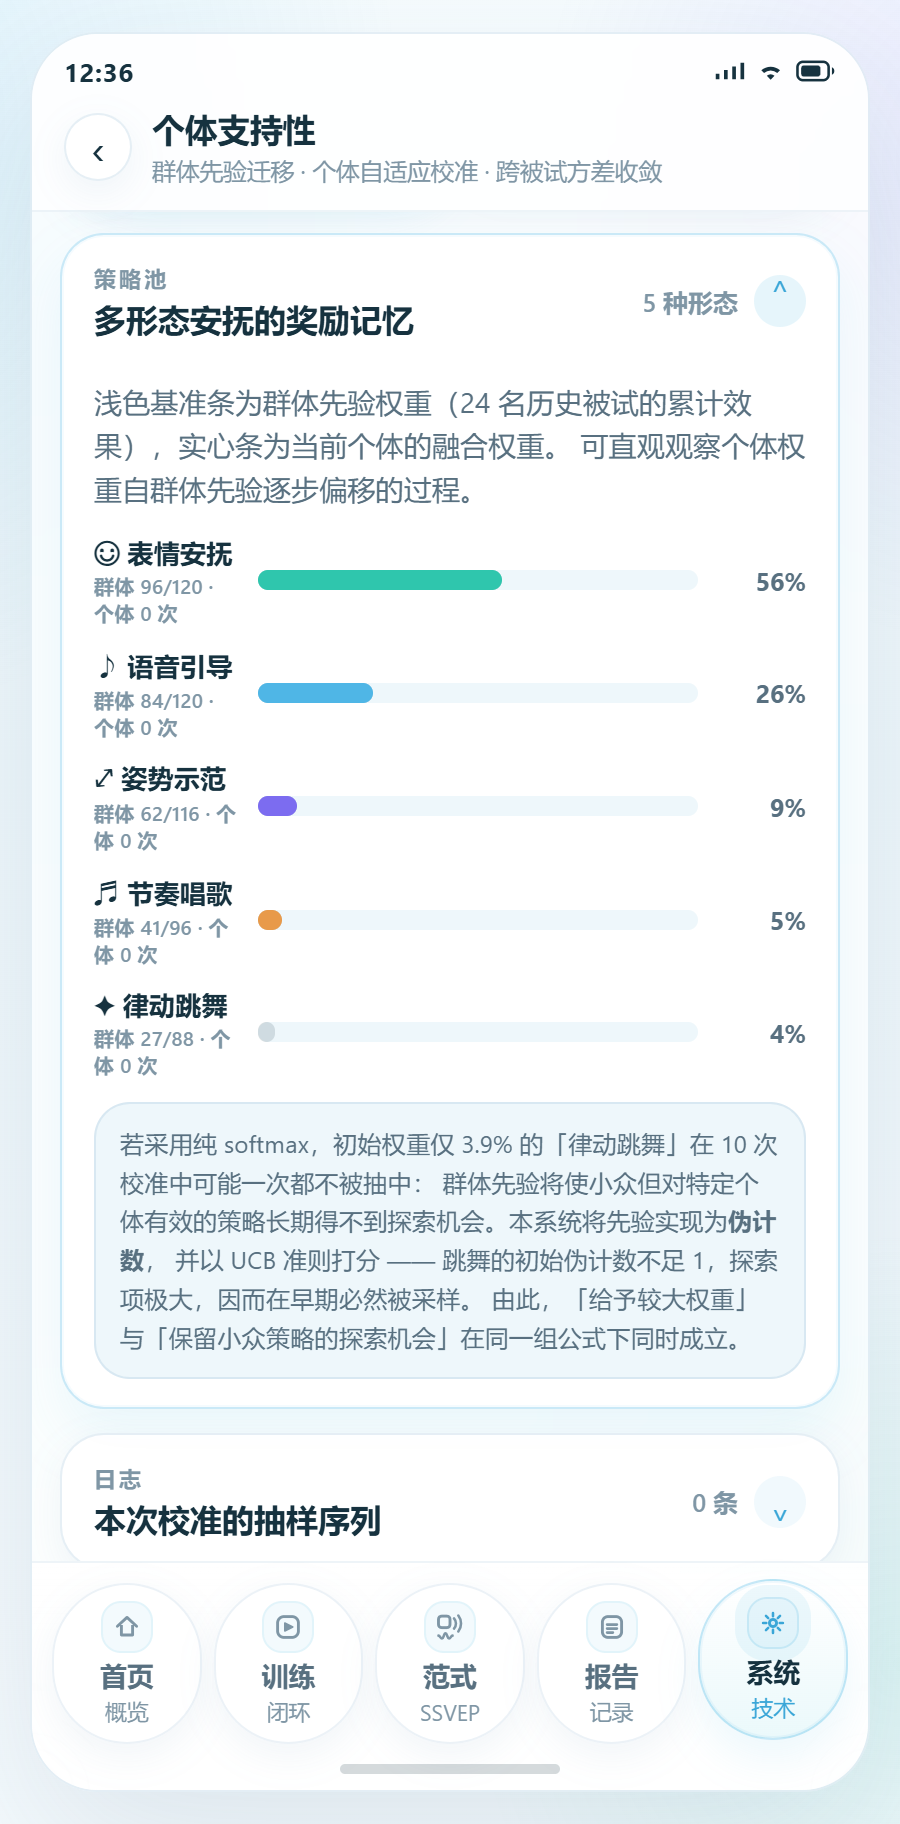
\includegraphics[width=\textwidth]{figures/06c-comfort-prior.png}
  \caption{接入时：群体先验权重}
\end{subfigure}
\hfill
\begin{subfigure}{0.42\textwidth}
  \centering
  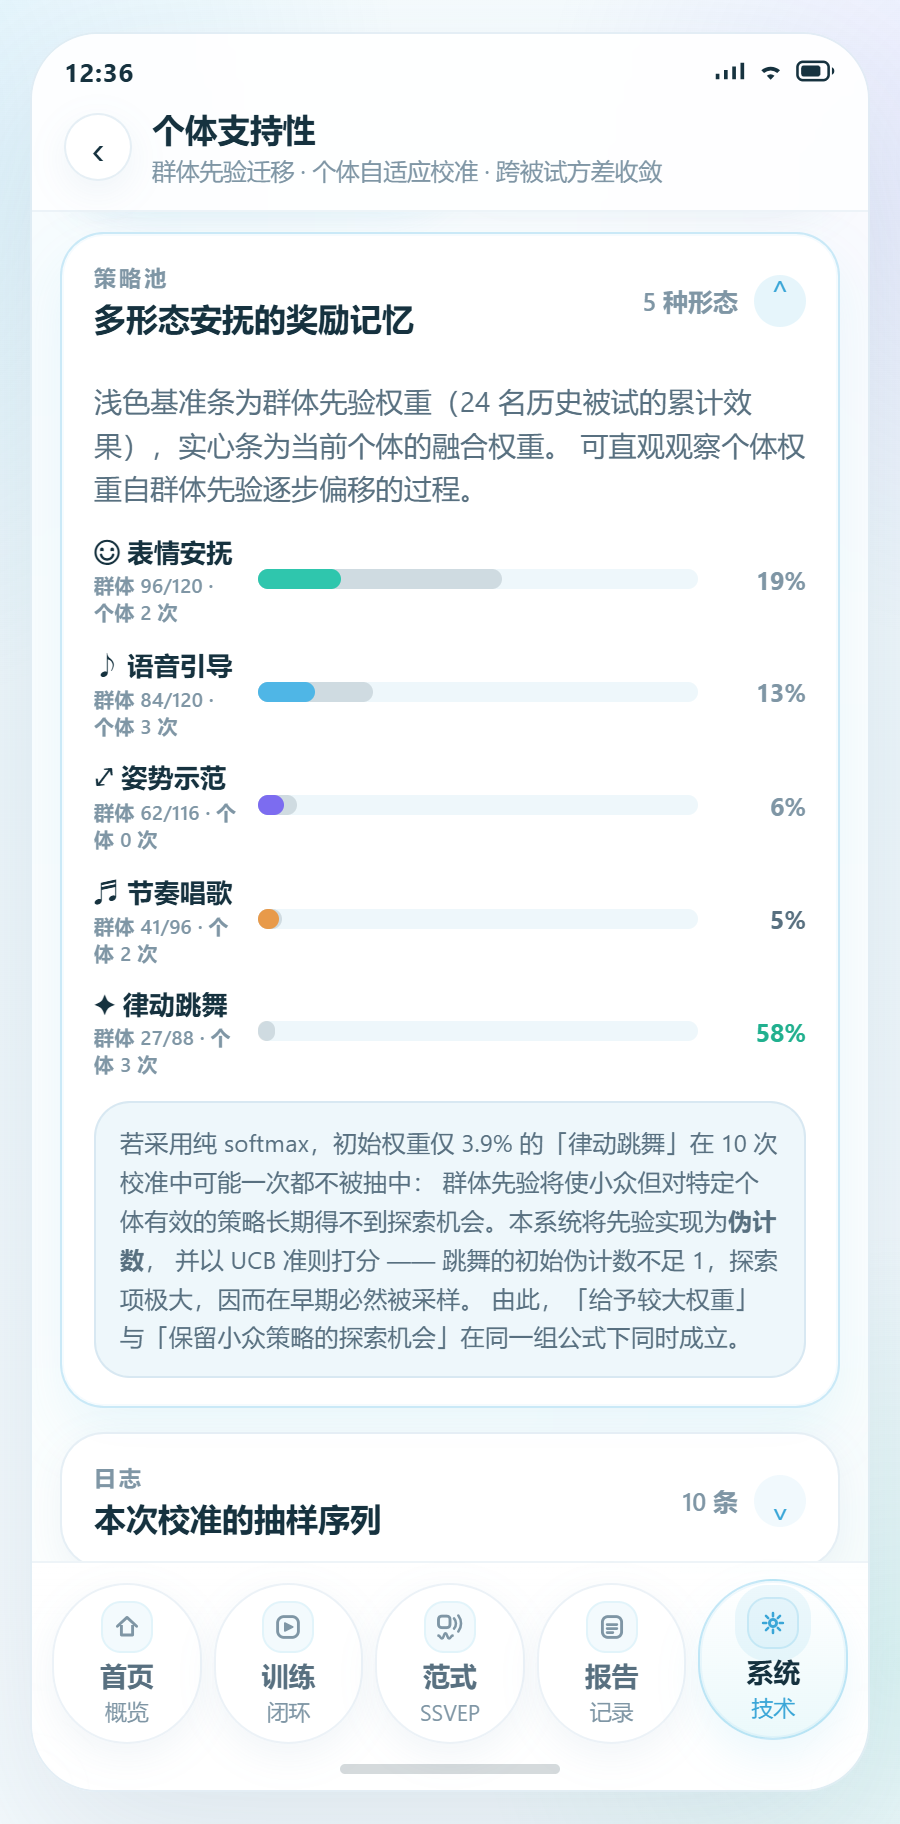
\includegraphics[width=\textwidth]{figures/06d-comfort-shifted.png}
  \caption{10 次反馈后：个体权重已迁移}
\end{subfigure}
\caption{多形态安抚的奖励记忆。浅色基准条为群体先验，实心条为当前个体的融合权重}
\end{figure}

\begin{table}[htbp]
\centering
\caption{「非典型型」个体的权重迁移}
\begin{tabular}{@{}l c c c@{}}
\toprule
\sffamily\bfseries 形态 & \sffamily\bfseries 群体先验 & \sffamily\bfseries 10 次反馈后 & \sffamily\bfseries 变化 \\
\midrule
表情安抚 & \textbf{56\%} & 19\% & $\downarrow$ \\
语音引导 & 26\% & 13\% & $\downarrow$ \\
姿势示范 & \phantom{0}9\% & \phantom{0}6\% & $\downarrow$ \\
节奏唱歌 & \phantom{0}5\% & \phantom{0}5\% & --- \\
律动跳舞 & \phantom{0}4\% & \textbf{58\%} & $\uparrow\uparrow$ \\
\bottomrule
\end{tabular}
\end{table}

群体先验认为「表情安抚」最有效（56\%），但对这名非典型个体而言，真正有效的是「律动跳舞」。\textbf{经过 10 次反馈，跳舞的权重从 4\% 跃升至 58\%，反超表情成为首选策略}——个体自适应成功推翻了群体先验。

\subsection{一个不易察觉的陷阱，以及它的解法}

\begin{warnbox}
\textbf{纯 softmax 会饿死小众策略。} 若直接按 softmax 权重抽样，初始权重仅 3.9\% 的「律动跳舞」在 10 次校准中\textbf{很可能一次都不会被抽中}——那么上一节的权重迁移\textbf{根本不会发生}。群体先验将使小众但对特定个体有效的策略永远得不到探索机会。这是一个隐蔽却致命的公平性缺陷。
\end{warnbox}

本系统的解法是：\textbf{把先验实现为伪计数，并以 UCB 准则打分}。

\[
\mathrm{score}(s) = \underbrace{\frac{n_s^{\text{prior}}\cdot p_s^{\text{prior}} + h_s}{n_s^{\text{prior}} + t_s}}_{\text{融合命中率}}
\;+\; \underbrace{c\sqrt{\frac{\ln (k+2)}{n_s^{\text{prior}} + t_s}}}_{\text{探索项}},
\qquad c = 0.35
\]

跳舞的初始伪计数不足 1（$n^{\text{prior}} \approx 0.59$），使得探索项的分母极小、\textbf{探索奖励极大}，因而在早期\textbf{必然被采样到}。于是：

\begin{keybox}
\textbf{「给予较大权重」与「保留小众策略的探索机会」这两个看似矛盾的目标，由同一组公式同时满足。}
\end{keybox}

\subsection{疲劳与安抚的耦合}

安抚策略的选择并非只看命中率，还受\textbf{疲劳指数}约束。「重度疲劳型」画像演示了这一点：高唤醒度的唱歌与跳舞反而会加重疲劳，因此系统会收敛到低唤醒度的语音引导与姿势示范。这条通路即：\textbf{脑电 $\to$ 疲劳指数 $\to$ AI 决策 $\to$ 安抚策略选择}。

\shot{06e-comfort-log.png}{0.40\textwidth}{UCB 抽样日志：可逐条核查 10 次校准中系统实际抽取了哪些策略、命中与否}

\newpage
% =====================================================================
\section{普适性扩展}

\begin{keybox}
\textbf{对应需求。} \req{功能加上普适性的扩展}。
\end{keybox}

普适性扩展在本系统中\textbf{落实在三个不同层面}，而非一句口号。

\subsection{硬件层：一套设备，三种范式}

主动式（运动想象）与反应式（SSVEP）两种范式，\textbf{共用同一套 8 通道无线采集硬件}，区别仅在于启用哪些通道子集：

\begin{table}[htbp]
\centering
\caption{同一硬件支撑不同范式}
\begin{tabularx}{\textwidth}{@{}l l X@{}}
\toprule
\sffamily\bfseries 范式 & \sffamily\bfseries 启用通道 & \sffamily\bfseries 额外硬件 \\
\midrule
主动式 · 运动想象 & 运动区 C3 / Cz / C4 / CP3 / CP4（5 通道） & 无 \\
反应式 · SSVEP    & 枕区 O1 / Oz / O2（3 通道）               & 仅需启停刺激器 \\
被动式 · 状态监测 & 复用上述通道估计疲劳指数                  & 无 \\
\bottomrule
\end{tabularx}
\end{table}

\textbf{切换范式仅需切换通道子集并启停刺激器，无需更换硬件}——普适性扩展由此在硬件层得到落地。

\subsection{患者层：能力受限时的替代通道}

不同患者的残余能力差异极大，系统因此不依赖单一输入通道：

\begin{itemize}[itemsep=3pt, topsep=4pt]
  \item \textbf{具备残余运动想象能力}者，走主动式范式；
  \item \textbf{重度运动障碍或康复早期}患者，认知负担低、基本免训练的\textbf{反应式 SSVEP} 提供备用通道；
  \item \textbf{面部感觉运动受损}者，其表情表达受限，此时系统以\textbf{疲劳指数与肌电通道交叉校验}；
  \item 面部受限于表情表达能力、语音受限于言语功能——\textbf{任一通道受限时，其余通道可承接其意图带宽}。
\end{itemize}

\subsection{算法层：对个体差异的自适应}

第 10--12 章所述的群体先验与个体自适应机制，本身即是最强的普适性扩展：\textbf{它使系统不必为每一位新患者重新训练模型，也不会因个体偏离群体分布而失效}。跨被试标准差由 $\sigma = 9.2\%$ 收敛至 $3.1\%$，正是普适性在算法层的量化证明。

\shot{07-wireless.png}{0.40\textwidth}{无线采集页：8 通道半干电极，同一套硬件通过切换通道子集支撑三种范式}

\newpage
% =====================================================================
\section{主动 / 被动范式与无线采集}

\begin{keybox}
\textbf{对应需求（董老师补充）。} \req{主动被动}——无线采集、范式的形式体现。
\end{keybox}

\subsection{先厘清一个术语混淆}

\begin{warnbox}
脑机接口领域的「主动 / 被动」存在\textbf{两个彼此正交的含义}，混用会导致论证失焦。本系统明确区分：

\begin{itemize}[itemsep=2pt, topsep=3pt]
  \item \textbf{维度一 · 范式}——解码何种脑活动。按 Zander \& Kothe (2011) 的三分法：主动式 / 反应式 / 被动式；
  \item \textbf{维度二 · 采集形态}——被试需佩戴何种设备。从湿电极脑帽，到耳内电极，直至完全不采脑电。
\end{itemize}

二者可自由组合：运动想象（\textbf{主动式范式}）可配耳内电极（\textbf{免佩戴形态}）；SSVEP（\textbf{反应式范式}）亦可配湿电极帽（\textbf{需佩戴形态}）。因此\textbf{「免佩戴」与「被动式范式」分属不同维度，需分别论证}。
\end{warnbox}

\subsection{三种范式在本系统中的对应实现}

\begin{table}[htbp]
\centering
\caption{范式三分法与本系统的对应实现（3 / 3 已实现）}
\begin{tabularx}{\textwidth}{@{}l X l@{}}
\toprule
\sffamily\bfseries 范式 & \sffamily\bfseries 在本系统中的实现 & \sffamily\bfseries 位置 \\
\midrule
主动式 & 运动想象——患者主动产生抬手 / 伸肘 / 握拳 / 放松四类意图 & 训练页环节二 \\
反应式 & SSVEP——注视闪烁目标即可解码，无需运动想象 & 范式页 \\
被动式 & 疲劳指数——系统读取患者状态，患者\textbf{不发出任何指令} & 贯穿 AI 决策与安抚策略 \\
\bottomrule
\end{tabularx}
\end{table}

\begin{keybox}
\textbf{SSVEP 属反应式，不属被动式。} 使用者仍在\textbf{有意识地选择注视对象}，因此按 Zander \& Kothe 的三分法应归入反应式。真正的被动式是系统读取使用者状态、而使用者不发出指令——在本系统中即\textbf{疲劳指数驱动训练强度自适应}这条通路。三种范式均有对应实现，共同构成一套完整的\textbf{混合式脑机接口}。
\end{keybox}

\subsection{被动式范式：读取客观状态，而非「不知情采集」}

被动式范式在康复场景中的价值，是\textbf{以不可伪装的客观状态驱动闭环自适应训练}。但它极易被误读为「趁患者不知情偷偷采集」。这是\textbf{两个彼此正交的概念}，本系统对二者的立场截然不同，特此挑明这条界线。

\begin{keybox}
\textbf{「被动」界定的是患者未参与指令发出，与患者是否知情、是否佩戴设备无关。} 疲劳、认知负荷、注意力这类状态，患者并未主动「发出」它们，但完全可以清楚地「知道」系统正在读取它们。因此\textbf{被动范式}（是否发指令）与\textbf{不知情采集}（是否被告知）分属两根不同的轴。
\end{keybox}

\textbf{为什么被动信号能给出更客观的结果？} 被动信号的价值在于它是\textbf{不自主}的——患者无法用意志掩盖前额叶脑电中的疲劳特征。这使它绕开了自述评估的三重系统性偏差：为讨好治疗师而少报疲劳、卒中后失语或认知障碍导致难以准确表达、以及主观标度因人而异。被动信号因此提供了一份可校正甚至替代自述的\textbf{客观基准（ground truth）}，这正是它「更真实」的技术来源。该客观状态进入 AI 康复决策后，驱动训练强度、力度上限与安抚策略的动态调整，使患者稳定在「有挑战但不过载」的最佳训练区间——而主动参与正是神经可塑性得以发生的前提（见第 5 章双通道架构）。

\begin{warnbox}
\textbf{「更真实」来自信号的不自主，而非患者的不知情。} 患者在\textbf{知情同意之后}，其疲劳信号依然一样真实——因为他本就压不住这个不自主的信号。换言之，\textbf{隐瞒采集在结果的真实性上一分不多买，只徒增伦理风险}。被动式状态监测的全部技术收益，均可在完全知情、采集状态常驻可见、可一键关闭的前提下\textbf{无损获得}。
\end{warnbox}

采集形态的「无感」程度，是与范式正交的另一根轴（即第 14.1 节的「采集形态」轴，其伦理含义见第 15 章条目「无感采集与知情同意」）：采集越无感（耳内电极、非接触电极），患者越难自觉正在被读取状态，知情同意越容易被架空。故本系统规定，免佩戴与被动通道\textbf{必须由使用者显式开启、采集状态常驻可见、可随时一键关闭，不得默认启用}。

\begin{keybox}
\textbf{一句话界定。} 被动范式（读取客观状态）与不知情采集（架空知情同意）是两件正交的事——\textbf{本系统采用前者，并明确防范后者}。二者的技术收益与伦理边界因此可以同时成立。
\end{keybox}

\subsection{SSVEP 反应式范式}

\begin{table}[htbp]
\centering
\caption{SSVEP 四目标的频率-相位联合调制}
\begin{tabular}{@{}l c c l@{}}
\toprule
\sffamily\bfseries 目标 & \sffamily\bfseries 频率 & \sffamily\bfseries 相位 & \sffamily\bfseries 映射动作 \\
\midrule
抬手 & \phantom{0}8.0 Hz & $\varphi = 0$        & 肩部辅助抬升 \\
伸肘 & 10.0 Hz & $\varphi = \pi/2$    & 肘部屈伸 \\
握拳 & 12.0 Hz & $\varphi = \pi$      & 手部抓握 \\
放松 & 15.0 Hz & $\varphi = 3\pi/2$   & 放松恢复 \\
\bottomrule
\end{tabular}
\end{table}

枕区 O1 / Oz / O2 三通道脑电中浮现同频稳态响应，功率谱呈现基频与二次谐波峰，FBCCA 输出各候选频率的相关系数 $\rho$。信息传输率按 Wolpaw 公式实算：

\[
\text{ITR} = \mathbf{39.2}\ \text{bits/min}
\qquad (N = 4,\; P = 0.95,\; T = 2.5\,\text{s})
\]

\begin{warnbox}
\textbf{光敏安全。} $8\sim 15$ Hz 的闪烁落在光敏性癫痫的风险频段（$3\sim 30$ Hz），因此该模块的闪烁\textbf{默认关闭}，必须由使用者\textbf{显式点击开启}；同时采用低对比度亮度调制，并遵循系统的 \texttt{prefers-reduced-motion} 设置。深链参数只预选目标，\textbf{不代替使用者作出同意}。
\end{warnbox}

\shot{03-ssvep.png}{0.40\textwidth}{SSVEP 范式页：四目标频率-相位联合调制；闪烁刺激默认关闭，需显式开启}

\subsection{无线采集与端到端时延预算}

首页指标「响应延迟 176ms $\le$ 200ms」并非一个孤立数值，而\textbf{由五个环节构成，各环节均有明确的物理依据}：

\begin{table}[htbp]
\centering
\caption{端到端时延预算分解（无线 BLE 方案）}
\begin{tabularx}{\textwidth}{@{}l c X@{}}
\toprule
\sffamily\bfseries 环节 & \sffamily\bfseries 耗时 & \sffamily\bfseries 物理依据 \\
\midrule
脑电采集与打包   & 64ms & 250Hz $\times$ 16 样本/包，对应 64ms 的包周期 \\
BLE 无线传输     & 30ms & BLE 5.0 连接间隔 15ms，可靠投递上界 $= 15 \times 2$ \\
预处理与解码     & 42ms & $6\sim 40$Hz 带通 + 50Hz 陷波 + CSP / FBCCA + LDA 前向 \\
AI 康复决策      & 11ms & 规则引擎与轻量策略网络，以查表运算为主 \\
指令下发与伺服启动 & 29ms & CAN 下发 + 伺服启动死区 \\
\midrule
\sffamily\bfseries 合计 & \sffamily\bfseries 176ms & 上限 200ms，\textbf{剩余余量 24ms} \\
\bottomrule
\end{tabularx}
\end{table}

\begin{keybox}
\textbf{无线的代价被诚实地标了出来。} 无线链路（采集打包 + BLE 传输）合计 94ms，\textbf{占整个时延预算的 53.4\%}。若改用有线方案，总时延可降至 114ms——即\textbf{无线的代价是 $+62$ms}。系统并未回避这一代价，而是明确展示：在 200ms 的预算内，无线方案仍留有 24ms 余量，因此\textbf{为了患者的活动自由度，这笔代价是值得付的}。

同时，正因无线链路存在丢包与重传风险，\textbf{过力保护环路（8ms）被刻意放在本地 MCU 上，不经过无线链路}（见第 8 章）。
\end{keybox}

\shot{08-acquisition.png}{0.40\textwidth}{范式与采集形态页：明确区分「范式」与「采集形态」两个正交维度}

\newpage
% =====================================================================
\section{伦理性问题}

\begin{keybox}
\textbf{对应需求（董老师补充）。} \req{伦理性问题}。
\end{keybox}

\subsection{设计原则：每一条伦理主张都必须可核查}

本系统的伦理页与常见的「伦理声明」有一个根本区别：\textbf{每一条伦理主张都标注了它在代码中的可核查实现位置；尚未达成之处，如实列为「部分实现」，不加掩饰}。

\begin{table}[htbp]
\centering
\caption{伦理措施总览（共 12 条）}
\begin{tabular}{@{}l c@{}}
\toprule
\sffamily\bfseries 状态 & \sffamily\bfseries 条目数 \\
\midrule
已实现   & 9 \\
部分实现 & 3 \\
规划中   & 0 \\
\bottomrule
\end{tabular}
\end{table}

\subsection{九条已实现的伦理措施}

\begin{table}[htbp]
\centering
\caption{已实现的伦理措施及其实现证据}
\begin{tabularx}{\textwidth}{@{}l X@{}}
\toprule
\sffamily\bfseries 条目 & \sffamily\bfseries 主张与实现证据 \\
\midrule
光敏性癫痫防护 & 不得让使用者在毫无预警的情况下暴露于致病性视觉刺激。SSVEP 的 $8\sim 15$Hz 闪烁落在 $3\sim 30$Hz 风险频段，因此\textbf{默认关闭}，须显式开启；采用低对比度亮度调制；遵循 \texttt{prefers-reduced-motion} \\
数据不出端     & 脑电数据不存在离开本设备的传输通道。伦理页\textbf{读取浏览器资源计时接口，实测本应用发出的跨域请求数量为 0}——该结论由页面运行时实测得出，而非静态声明 \\
数据最小化     & 仅采集完成任务所必需的通道与时段 \\
低置信度拒识   & 置信度不足时拒绝执行，而非勉强给出动作。「放松」意图的安全结论为「需复核」即此机制的体现 \\
过力保护与物理安全 & 力度指令经硬阈钳制（软阈 72\% / 硬阈 85\%），环路时延 8ms，运行于本地 MCU，不经无线链路 \\
人在回路       & 治疗师可随时中断，系统不具备无人监督下的自主执行权 \\
决策可解释     & AI 决策的每一条方案均附其依据（意图、姿态评分、疲劳指数、误操作风险） \\
失效安全降级   & WebGL 不可用时三维面板降级为静态说明，其余功能不受影响，不白屏 \\
不夸大宣传     & 全部信号为仿真合成数据，页面多处明示「合成数据 · 非临床结论」 \\
\bottomrule
\end{tabularx}
\end{table}

\subsection{三条「部分实现」——如实列出缺口}

\begin{warnbox}
以下三条\textbf{尚未完全达成}。系统选择如实列出，而非隐去：

\begin{itemize}[itemsep=4pt, topsep=4pt]
  \item \textbf{算法公平性}——跨被试标准差虽已由 $\sigma = 9.2\%$ 降至 $3.1\%$，但\textbf{强先验对非典型个体的响应仍然迟缓}：如第 12 章所述，「非典型型」个体约需 8 次反例才能推翻群体先验对「表情」策略的惯性。这段延迟期内，系统对该个体的适配是次优的。
  \item \textbf{无感采集与知情同意}——采集形态越是无感（如耳内电极），使用者越\textbf{难以意识到自己正在被采集脑电}。知情同意的形式设计尚未完成。
  \item \textbf{脆弱人群保护}——卒中患者、认知障碍者等脆弱人群的额外保护措施尚待细化。
\end{itemize}
\end{warnbox}

\begin{keybox}
\textbf{把缺口写出来，本身就是一种伦理实践。} 一个只列成绩、不列缺口的伦理页，其可信度反而更低。本系统选择让「部分实现」的三条与「已实现」的九条并列展示，并各自标注具体的差距所在。
\end{keybox}

\shot{09-ethics.png}{0.40\textwidth}{伦理与安全页：12 条措施，9 条已实现、3 条部分实现；外部请求实测为 0 个}

\newpage
% =====================================================================
\section{技术架构与分发}

\subsection{四层架构}

\begin{table}[htbp]
\centering
\caption{系统四层架构}
\begin{tabularx}{\textwidth}{@{}l X@{}}
\toprule
\sffamily\bfseries 层 & \sffamily\bfseries 组成 \\
\midrule
感知层     & EEG 模拟输入、RGB / NIR / ToF、力觉与触觉采样 \\
意图理解层 & 运动意图分类、姿态评分、疲劳与风险估计 \\
决策控制层 & AI 康复决策、机械臂轨迹规划、过力保护规则 \\
反馈评估层 & 压力 / 振动 / 位置感反馈、训练报告、个体化记忆更新 \\
\bottomrule
\end{tabularx}
\end{table}

\subsection{技术栈}

React 18 + TypeScript + Vite 5；三维仿真使用 three.js \textbf{程序化建模}（无外部模型文件）。

\begin{keybox}
\textbf{应用不请求任何外部资源}——无字体外链、无图片外链、无 CDN 依赖，\textbf{加载后完全离线可用}。这既是工程决策，也是第 15 章「数据不出端」伦理主张的技术前提。
\end{keybox}

\subsection{分发方式}

\begin{itemize}[itemsep=3pt, topsep=4pt]
  \item \texttt{npm run build}——静态站点，产出至 \texttt{dist/}；
  \item \texttt{npm run build:single}——\textbf{单文件 HTML}，JS 与 CSS 全部内联，双击即可离线打开；
  \item \texttt{npm run build:apk}——Android APK（需 Android SDK）。
\end{itemize}

\newpage
% =====================================================================
\appendix
\section*{附录 A\quad 需求对照表}
\addcontentsline{toc}{section}{附录 A\quad 需求对照表}
\markboth{附录 A}{附录 A}

下表将竞赛需求书（\texttt{CLAUDE.md}）中的每一条关键要求，映射至本说明书的对应章节与系统中的实现位置。

\begin{longtable}{@{}p{0.30\textwidth} c p{0.42\textwidth}@{}}
\toprule
\sffamily\bfseries 需求条目 & \sffamily\bfseries 章节 & \sffamily\bfseries 实现位置 \\
\midrule
\endhead
七环节闭环主流程       & 第 3--9 章 & 训练页 · 七步手风琴 \\
首页关键指标（4 项）   & 第 1 章    & 首页 · 关键指标卡，均可下钻 \\
光电模块改写用途       & 第 5 章    & 训练页环节三 · RGB / NIR / ToF \\
强化脑电交互模块       & 第 4 章    & 训练页环节二 · 四类意图按钮 \\
新增 AI 康复决策模块   & 第 6 章    & 训练页环节四 \\
改造机器人动作响应模块 & 第 7 章    & 训练页环节五 · 三个训练动作 \\
新增触觉反馈闭环模块   & 第 8 章    & 训练页环节六 · 三类反馈 + 过力保护 \\
新增训练报告生成模块   & 第 9 章    & 报告页 · 八项指标 + Word 导出 \\
固定演示流程           & 第 2 章    & 首页「开始演示」\\
3D 建模仿真交互        & 第 7 章    & three.js 程序化机械臂，可拖动旋转 \\
\midrule
普适性的扩展           & 第 13 章   & 硬件层 / 患者层 / 算法层三个层面 \\
机器人多形态情绪安抚   & 第 12 章   & 个体支持性页 · 策略池（表情/语言/姿势/唱歌/跳舞）\\
奖励性增强 · 记忆功能  & 第 11 章   & 个体支持性页 · 群体先验与个体校准 \\
\midrule
个体的支持性（董）     & 第 10 章   & 个体支持性页 · $\sigma$ 9.2\% $\to$ 3.1\% \\
主动 / 被动（董）      & 第 14 章   & 范式与采集形态页、无线采集页、SSVEP 页 \\
伦理性问题（董）       & 第 15 章   & 伦理与安全页 · 12 条措施 \\
\bottomrule
\end{longtable}

\section*{附录 B\quad 数据声明}
\addcontentsline{toc}{section}{附录 B\quad 数据声明}
\markboth{附录 B}{附录 B}

\begin{warnbox}
本系统中的\textbf{全部脑电信号、被试队列、准确率与时延数值均为仿真合成数据}，用于系统功能验证与竞赛演示。

\begin{itemize}[itemsep=3pt, topsep=4pt]
  \item 它们\textbf{不构成任何临床结论}，亦\textbf{不可作为诊断或治疗依据}；
  \item 24 名被试的队列由固定种子的确定性伪随机数生成器构造，其均值与标准差从数据点上真实算出，\textbf{与文案所述数值严格一致}；
  \item 时延预算中的各环节耗时均给出了物理依据（采样率、BLE 连接间隔、滤波器阶数等），但\textbf{未经真实硬件实测}；
  \item 训练报告在本机生成，\textbf{未经由网络上传}。
\end{itemize}
\end{warnbox}

\vfill
\begin{center}
\color{brandgrey}\sffamily\small
脑机协同康复机械臂闭环可视化系统 · 产品说明书 · v1.0
\end{center}

\end{document}
